\documentclass[10pt]{beamer}

\usetheme{metropolis}
\usepackage{appendixnumberbeamer}

\usepackage{booktabs}
\usepackage[scale=2]{ccicons}
\usepackage{graphicx}
\usepackage{hyperref}
\usepackage{circuitikz}
\usepackage{pdflscape}
\usepackage{smartdiagram}

\usepackage{color}
\usepackage{listings}

\lstset{
	basicstyle=\footnotesize\ttfamily,
    keepspaces=true,
    showstringspaces=false,
    language=PHP,
    commentstyle=\ttfamily,
}

\usepackage[OT4]{polski}
\usepackage[utf8]{inputenc}

\usepackage{pgfplots}
\usepgfplotslibrary{dateplot}

\usepackage{xspace}
\newcommand{\themename}{\textbf{\textsc{metropolis}}\xspace}

\setbeamertemplate{frame footer}{}
\setbeamertemplate{frame numbering}{}

\usetikzlibrary{shapes,arrows}

\tikzstyle{decision} = [diamond, draw, fill=blue!20, 
    text width=4.5em, text badly centered, node distance=3cm, inner sep=0pt]
\tikzstyle{block} = [rectangle, draw, fill=blue!20, 
    text width=5em, text centered, rounded corners, minimum height=4em]
\tikzstyle{line} = [draw, -latex']
\tikzstyle{cloud} = [draw, ellipse,fill=red!20, node distance=3cm,
    minimum height=2em]


\title{Wprowadzenie}

\subtitle{Projektowanie i programowanie systemów internetowych I}
\author{mgr inż. Krzysztof Rewak}
\date{\today}
\institute{Wydział Nauk Technicznych i Ekonomicznych \\ Państwowa Wyższa Szkoła Zawodowa im. Witelona w Legnicy}

\begin{document}

\maketitle

\begin{frame}{Plan prezentacji}
  \setbeamertemplate{section in toc}[sections numbered]
  \tableofcontents[hideallsubsections]
\end{frame}


\section{Ramowy plan semestru}

\begin{frame}{Planowany rozkład jazdy}
	Wykład 1: Wprowadzenie; dobór technologii projektowej
	
	Wykład 2: Zasady SOLID
	
	Wykład 3: KISS, DRY, YAGNI i inne
	
	Wykład 4: Czysty kod, część I
	
	Wykład 5: Czysty kod, część II
	
	Wykład 6: Czysty kod, część III
	
	Wykład 7: Praktyczny polimorfizm
\end{frame}

\begin{frame}{Planowany rozkład jazdy}
	Wykład 8: Progamowanie asynchroniczne
	
	Wykład 9: Wzorce projektowe: kreacyjne
	
	Wykład 10: Wzorce projektowe: strukturalne
	
	Wykład 11: Wzorce projektowe: operacyjne
	
	Wykład 12: Antywzorce projektowe
	
	Wykład 13: Programowanie ekstremalne
	
	Wykład 14: Praca w zespole programistycznym
	
	Wykład 15: Kolokwium zaliczeniowe
\end{frame}

\section{Warunki zaliczenia kursu}

\begin{frame}{Formy zajęć}
	\begin{figure}
		\resizebox{.5\linewidth}{!}{W + L}
	\end{figure}
	
	\ \\
	
	\textbf{wykład} - teoretyczna część kursu; przedstawienie wybranych zagadnień związanych z aplikacjami webowymi;
	
	\textbf{laboratorium} - praktyczna część kursu; praca zespołowa nad projektowaniem, implementacją oraz wdrożeniem projektu programistycznego.
\end{frame}

\begin{frame}{Warunki zaliczenia wykładu}
	Wykład kończy się egzaminem podsumowującym wiedzę przyswojoną w trakcie semestru. Egzamin - w zależności od liczby przystępujących osób - odbędzie się w formie pisemnej lub ustnej.
	
	Student, który otrzyma z projektu ocenę niedostateczną nie może podchodzić do egzaminu.
\end{frame}

\begin{frame}{Warunki zaliczenia wykładu}	
	Ponadto na wykładach:
	\begin{itemize}
		\item będzie sprawdzana lista obecności na zasadzie białej listy;
		\item będzie mierzona (pozytywna i negatywna) aktywność studentów.
	\end{itemize}
	
	Zachęcam do uczęszczania na wykłady.
\end{frame}

\begin{frame}{Ocena końcowa}
	\begin{figure}
		\resizebox{.66\linewidth}{!}{0.3W + 0.7L}
	\end{figure}
	
	Ocena niedostateczna z jednej formy rzutuje na ocenę niedostateczną za całość!
	
	Przykładowo:
	\begin{itemize}
		\item 3.0 E + 5.0 L = 4.4 $\Rightarrow$ \textbf{4.5}
		\item 4.5 E + 4.0 L = 4.15 $\Rightarrow$ \textbf{4.0}
		\item 2.0 E + 5.0 L = 4.1 $\Rightarrow$ \textbf{2.0}
	\end{itemize}
\end{frame}

\begin{frame}{Bonusy}	
	Osoby, które otrzymały ocenę z projektu \textbf{$p = 5.0$}, zostaną zwolnione z egzaminu z przepisaną oceną.
\end{frame}

\begin{frame}{Bonusy}	
	Wysoka frekwencja oraz aktywność na wykładach mogą rzutować na obniżenie progu przepisywanej oceny do $p \geq 4.5$ dla indywidualnych studentów.
\end{frame}

\begin{frame}{Bonusy}		
	W trakcie semestru organizowane będą dodatkowe zwolnienia z egzaminu w formie interaktywnych \emph{kartkówek} z bieżącego materiału.
	
	Student, który otrzyma najwięcej punktów z danej \emph{kartkówki}, zostanie zwolniony z egzaminu z przepisaną oceną z projektu.
\end{frame}

\begin{frame}{Bibliografia i ciekawe źródła}
  
	\begin{thebibliography}{9}
	
		\bibitem{cc}
		Robert C. Martin,
		\textit{Czysty kod. Podręcznik dobrego programisty},
		wyd. Helion
	
		\bibitem{wzorce}
		 Erich Gamma, Richard Helm, Ralph Johnson, John Vlissides,
		\textit{Wzorce projektowe. Elementy oprogramowania obiektowego wielokrotnego użytku },
		wyd. Helion
		
		\bibitem{php}
		PHP Design Patterns,
		\url{https://designpatternsphp.readthedocs.io/en/latest/}
	
	\end{thebibliography}

\end{frame}

\begin{frame}[standout]
	Pytania?
\end{frame}










\title{Dobór technologii projektowej}
\maketitle

\begin{frame}{\emph{¿Qué pasa?}}		
	Wybór języka programowania może być jedną z najważniejszych projektowych decyzji.
\end{frame}

\begin{frame}{\emph{No hablo inglés}}		
	Problematycznym podejściem może być sytaucja wprost ze znanego powiedzenia, w której mamy młotek i wszystko inne wygląda jak gwoździe.
	
	Często się okaże, że nasz ulubiony język czy framework - mimo wszystko! - nie będzie najlepszym z puli dostepnych rozwiązań.
\end{frame}

\section{Przegląd języków programowania}

\begin{frame}{Aplikacje webowe: backend}		
	Webowy backend jest podstawą większości nowoczesnych aplikacji, zarówno klasycznych webowych, jak i desktopowych, mobilnych i innych.
	
	SOAP, REST API, GraphQL czy też renderowanie HTML-owych widoków - każdy z tych sposobów komunikacji z backendem można zaimplementować w przynajmniej kilku różnych językach.
\end{frame}

\begin{frame}{Aplikacje webowe: backend}		
	\begin{figure}
		\centering
		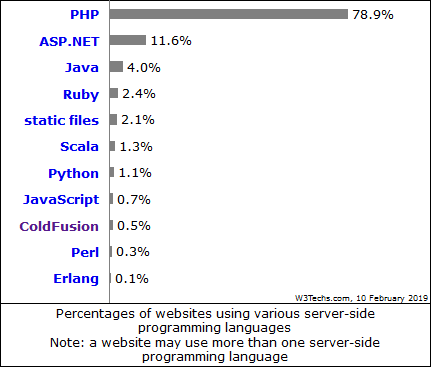
\includegraphics[width=.7\textwidth]{backend.png}
		\caption{\url{https://w3techs.com/technologies/overview/programming_language/all}}
	\end{figure}
\end{frame}

\begin{frame}{Aplikacje webowe: backend w PHP}		
	\textbf{PHP} jest naturalnym językiem programowania aplikacji webowych i powstał w tym celu w latach 90. ubiegłego wieku. 
	
	Cechy: obiektowy, dynamicznie i słabo typowany, interpretowany, wieloplatformowy, jeden proces na jedno zapytanie, mnóstwo frameworków.
\end{frame}

\begin{frame}{Aplikacje webowe: backend w Javie}		
	\textbf{Java} jest jednym z najczęściej używanych języków programowania na świecie, zarówno dla aplikacji mobilnych, desktopowych i webowych.
	
	Cechy: obiektowa, statycznie typowana, kompilowana, wielowątkowa, wieloplatformowa.
\end{frame}

\begin{frame}{Aplikacje webowe: backend w C\#}		
	\textbf{C\#} jest językiem stworzonym przez Microsoft do realizacji wielu zadań, a dzięki frameworkowi ASP.MVC i Core można tworzyć rozległe aplikacje webowe.
	
	Cechy: obiektowy, silnie typowany, kompilowany, wielowątkowy.
\end{frame}

\begin{frame}{Aplikacje webowe: backend w JavaScripcie}		
	\textbf{JavaScript} wykształcił się jako webowa technologia do wspomagania frontendu, jednak w ostatnich latach wyewoluował w pełnoprawny język backendowy.
	
	Cechy: wieloparadygmatowy, dynamicznie i słabo typowany, interpretowany, wieloplatformowy.
\end{frame}

\begin{frame}{Aplikacje webowe: backend w Go}		
	\textbf{Go} to odpowiedź Google na zapotrzebowanie rynku na szybki i wielowątkowy język programowania. 
	
	Cechy: statycznie i silnie typowany, kompilowalny, strukturalny, wielowątkowy.
\end{frame}

\begin{frame}{Aplikacje webowe: frontend}		
	\begin{figure}
		\centering
		
\includegraphics[width=.7\textwidth]{frontend.png}
	\end{figure}
\end{frame}

\begin{frame}{Aplikacje webowe: frontend w JavaScripcie}		
	\textbf{JavaScript} obecnie jest praktycznie monopolistą na rynku frontendowych aplikacji webowych. Dzięki dziesiątkom frameworków, każdy znajdzie wygodnie rozwiązanie.
	
	Cechy: wieloparadygmatowy, dynamicznie i słabo typowany, interpretowany, wieloplatformowy.
\end{frame}

\begin{frame}{Aplikacje desktopowe}		
	\begin{figure}
		\centering
		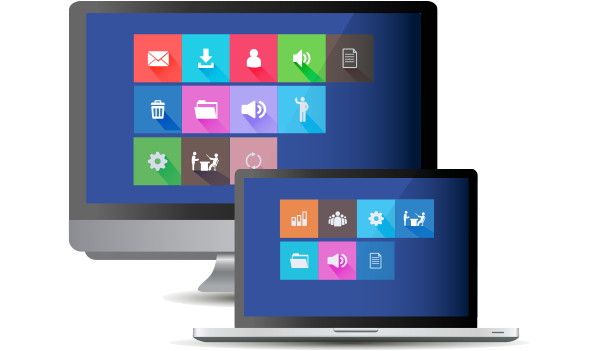
\includegraphics[width=.7\textwidth]{desktop.png}
	\end{figure}
\end{frame}

\begin{frame}{Aplikacje desktopowe: Java}		
	\textbf{Java} to jeden z najpopularniejszych języków programowania użytkownych aplikacji desktopowych. Z produktami pracy z frameworkami takimi jak Swing czy JavaFX spotkał się prawie każdy użytkownik komputerów z Windowsem czy Linuksem.
	
	Cechy: obiektowa, statycznie typowana, kompilowana, wielowątkowa, wieloplatformowa.
\end{frame}

\begin{frame}{Aplikacje desktopowe: C\#}		
	\textbf{C\#} z frameworkiem Microsoftu .NET jest podstawowym narzędziem do tworzenia windowsowych aplikacji.
	
	Cechy: obiektowy, silnie typowany, kompilowany, wielowątkowy.
\end{frame}

\begin{frame}{Aplikacje desktopowe: C++}		
	\textbf{C++} pozwoli na wykrzesanie z aplikacji największej wydajności, jednakże z pewnością będzie cięższy do opanowania. Popularnym frameworkiem do rozwiązań desktopowych wciąż jest Qt.
	
	Cechy: imperatywny, obiektowy, statycznie i silnie typowany, kompilowany, wielowątkowy.
\end{frame}

\begin{frame}{Aplikacje desktopowe: Python}		
	\textbf{Python} ma multum frameworków pozwalających na tworzenie aplikacji desktopowych. Jest to ulubiony język do rozwiązań naukowych i okołomatematycznych ze względu na rozległe repozytoria bibliotek.
	
	Cechy: interpretowany, dynamicznie i silnie typowany, obiektowy.
\end{frame}

\begin{frame}{Aplikacje desktopowe: JavaScript}		
	W \textbf{JavaScripcie} można również tworzyć aplikacje desktopowe za pomocą specjalistycznych frameworków takich jak Electron.
	
	Cechy: wieloparadygmatowy, dynamicznie i słabo typowany, interpretowany, wieloplatformowy.
\end{frame}

\begin{frame}{Aplikacje mobilne}		
	\begin{figure}
		\centering
		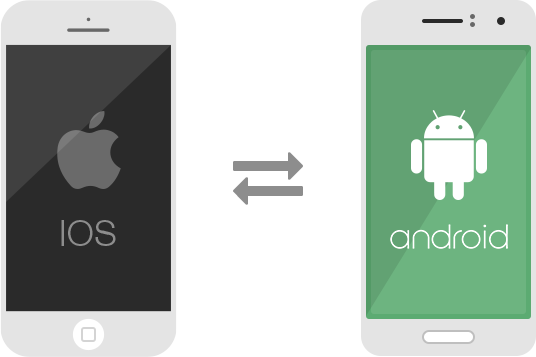
\includegraphics[width=.7\textwidth]{mobile.png}
	\end{figure}
\end{frame}

\begin{frame}{Aplikacje mobilne: Java}		
	\textbf{Java} to obecnie królowa języków programowania mobilnego. Android to obecnie ponad 80\% rynku smartfonów, a gigantyczna część wszystkich aplikacji napisana jest właśnie w Javie.
	
	Cechy: obiektowa, statycznie typowana, kompilowana, wielowątkowa, wieloplatformowa.
\end{frame}

\begin{frame}{Aplikacje mobilne: Kotlin}		
	\textbf{Kotlin} to wschodząca gwiazda sponsorowana przez JetBrains i Google, a wykrozystująca JVM. 
	
	Cechy: statycznie typowany, kompilowany, wielowątkowy, wieloplatformowy.
\end{frame}

\begin{frame}{Aplikacje mobilne: Swift}		
	\textbf{Swift} wyparł Objective-C i stał się podstawowym językiem programowania systemów opartych iOS.
	
	Cechy: wieloparadygmatowy, statycznie i silnie typowany, kompilowany.
\end{frame}

\begin{frame}{Aplikacje mobilne: JavaScript}		
	W \textbf{JavaScripcie} można również tworzyć aplikacje mobilne za pomocą specjalistycznych frameworków takich jak NativeScript.
	
	Cechy: wieloparadygmatowy, dynamicznie i słabo typowany, interpretowany, wieloplatformowy.
\end{frame}

\begin{frame}{Aplikacje przemysłowe}		
	\begin{figure}
		\centering
		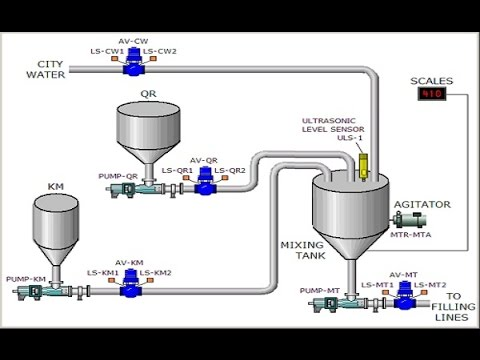
\includegraphics[width=.7\textwidth]{industrial.jpg}
	\end{figure}
\end{frame}

\begin{frame}{Aplikacje przemysłowe}		
	Przemysł rządzi się swoimi prawami. 
	
	Aplikacje przemysłowe będą najczęściej programowane w językach niskiego poziomu lub w specjalistycznych językach typu LD.
\end{frame}

\begin{frame}{Aplikacje przemysłowe}		
	\begin{figure}
		\centering
		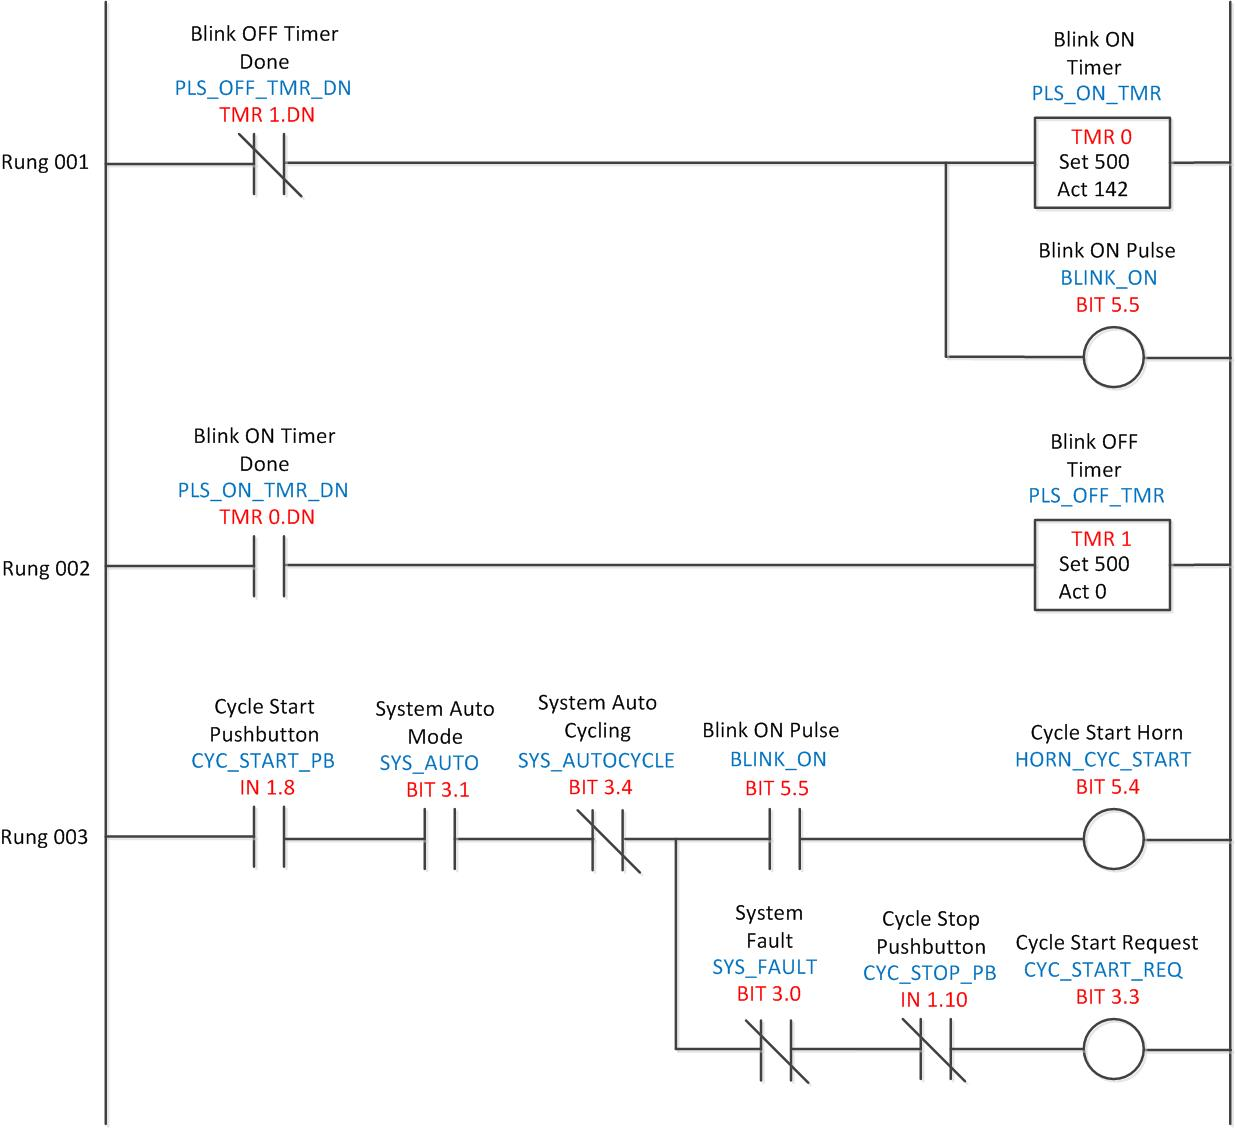
\includegraphics[width=.7\textwidth]{ladder.jpg}
	\end{figure}
\end{frame}

\section{Podsumowanie}

\appendix

\begin{frame}[standout]
	Pytania?
\end{frame}

\begin{frame}{}

	Kod prezentacji dostępny jest w repozytorium git pod adresem \texttt{https://bitbucket.org/krewak/pwsz-ppsi} \\ \ \\

	\begin{figure}
		\centering
		\href{https://bitbucket.org/krewak/pwsz-ppsi}{
			
\includegraphics[width=.15\textwidth]{../_template/bitbucket.png}
		}
	\end{figure}
	
	Wszystkie informacje dot. kursu dostępne są pod adresem \texttt{http://pwsz.rewak.pl/kursy/4} \\ \ \\

	\begin{figure}
		\centering
		\href{http://pwsz.rewak.pl/kursy/3}{
			
\includegraphics[width=.15\textwidth]{../_template/rewak.png}
		}
	\end{figure}

\end{frame}

\end{document}
